\section{Kapitel 1}

\subsection{Differentialgleichungen 1. Ordnung - Symbolische Lösungsverfahren}
\subsection{Gleichgewichtslösungen}
Die Gleichgewichtslösungen sind diejenigen Punkte, in welchen die Ableitung verschwindet:
\begin{equation*}
	\diffp{}{t}y(t) = 0
\end{equation*}
\subsection{Phasengerade und Integralkurven}
Bei der Phasengerade werden die Gleichgewichtslösungen in Funktion der Ableitung eingetragen. Dadurch kann die Stabilität eines Systems bestimmt werden. 

\subsection{Bifurkationen}
Gegeben ist eine autonome Differentialgleichung mit reellen Parametern.

\begin{equation*}
	\diffp{}{t}y(t) = f(a,y(t))
\end{equation*}

Suche die Gleichgewichtslösungen und unterscheide abhängig vom Parameter a in folgenden 3 Fällen:\\
\begin{itemize}
\item $a<0$
\item $a=0$
\item $a>0$
\end{itemize}
Für jeden dieser Fälle wird die Phasengerade gezeichnet und daraus kann man dann das entsprechende Bifurkationsdiagramm zeichnen. 

\begin{minipage}[h]{0.35\textwidth} 
	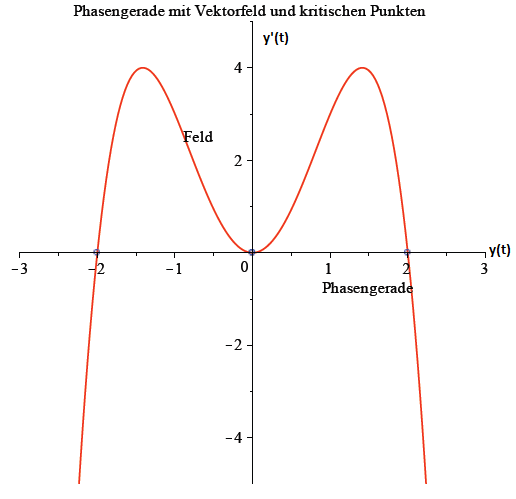
\includegraphics[width=1.0\textwidth]{images/Phasengerade.png}
\end{minipage}
\begin{minipage}[h]{0.35\textwidth}
	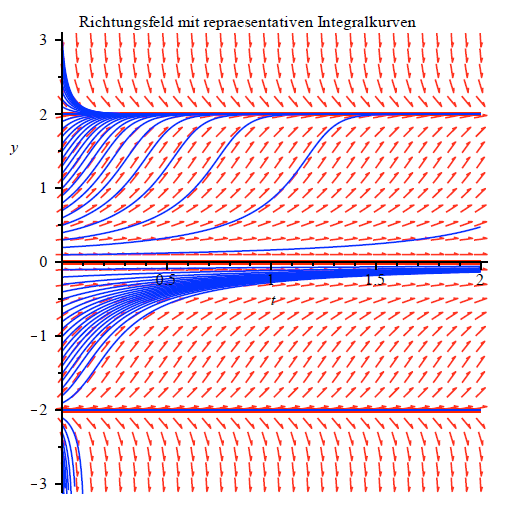
\includegraphics[width=1.0\textwidth]{images/Richtungsfeld.png}
\end{minipage}
\begin{tabular}{p{1.8cm}p{5cm}}
	$y(t) = -2$: & instabil \\
	$y(t) = 0$: & semistabil\\
	$y(t) = 2$: & asymtotisch stabil\\
\end{tabular}

\subsection{Bifurkationsdiagramm}
\begin{minipage}[h]{0.35\textwidth}
\[y'=y(a-y)\]
Kritische Punkte in Abhängikeit von $a$\\
\begin{tabbing}
Ausgezogen: \= Asymptotisch Stabil\\
Gestrichelt: \> Instabil\\
Zentrum: \> Semistabil\\
\end{tabbing}
\end{minipage}
\begin{minipage}[h]{0.35\textwidth}
	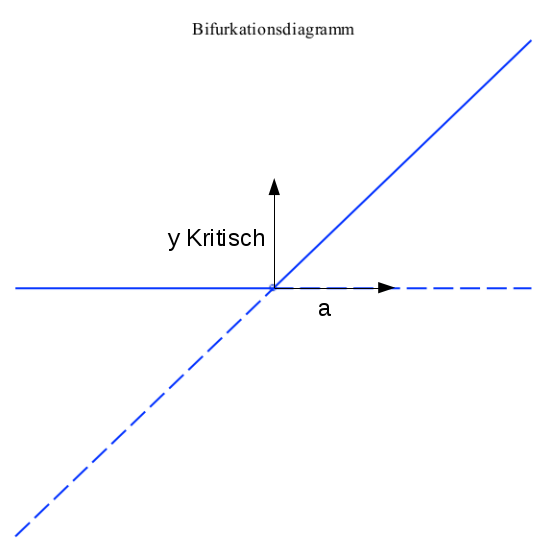
\includegraphics[width=1.0\textwidth]{images/Bifurkationsdiagramm.png}
\end{minipage}

\subsubsection{Allgemein 1. Ordnung}
\[ \dfrac{d}{dt}y(t)=f(t,y(t)) \qquad y(t_0)=y_0 \]
Eindeutige Lösung $\varphi(t)$ im Intervall falls $f(t,y(t))$ und $\dfrac{d \; f(t,y(t))}{dt}$ stetig im Intervall.

\subsection{Lineare homogene autonome DGL 1. Ordnung}
\[ \dfrac{d}{dt}y(t)+ay(t)=0 \qquad y(t_0)=y_0 \]
\begin{tabular}{ll}
Ansatz: & $y(t) = e^{\lambda t}$\\
Einsetzen in DGL: & $\lambda e^{\lambda t} + ae^{\lambda t} = 0$\\
Charakteristisches Polynom: & $\lambda = -a$\\
Allgemeine Lösung: & $y(t) = ce^{-ax}$\\
\multicolumn{2}{l}{Freiheitsgrad c mit Anfangswert bestimmen} \\
\end{tabular}

\subsection{Lineare inhomogene autonome DGL 1. Ordnung}
\[ \dfrac{d}{dt}y(t)+ay(t) = g(t) \]
Den inhomogenen Ansatz möglichst gleich der Inhomogenität $g(t)$ wählen, aber so dass $y_P$ linear unabhängig von der homogenen Lösung $y_H$ ist. (Siehe dazu die Tabelle für lineare inhomogene Gleichungen 2.Ordnung). \\

\paragraph{Vorgehen}~\\
\begin{tabularx}{\linewidth}{lX}
1. Schritt: & Einsetzen in inhomogene DGL und Koeffizienten mit Hilfe des Koeffizientenvergleichs bestimmen. $\rightarrow y_p(t)$\\
2. Schritt: & $y(t) = y_H(t)+y_P(t)$ \\
\end{tabularx}


\newpage
\subsection{Lösungsformeln 1. Ordnung}
\subsubsection{Lineare DGL}
\begin{tabular}{p{6cm}p{2cm}p{0.2cm}p{3.8cm}p{6.5cm}}
\textbf{Form:} \quad $y'(t) + p(t) \cdot y(t) = g(t)$ &
\textbf{Vorgehen:} &
1. & $\mu(t)$ berechnen: & $\mu(t) = e^{\int p(t) dt}$ \\ &&
2. & L"osung: & $y(t) = \frac{1}{\mu(t)} \cdot ( \int \mu(t) g(t) dt +c)$ \\ &&
\end{tabular}
Lösung existiert und eindeutig falls $p(t)$ und $g(t)$ stetig.\\
\textbf{Bsp}: $t^3 \cdot y'(t) + 4 t^2 \cdot y(t) = e^{-t} \quad \Longrightarrow \quad y'(t) + \underbrace{4 \frac{1}{t}}_{p(t)} \cdot y(t) = \underbrace{\frac{1}{t^3} e^-t}_{g(t))}$

\subsubsection{Separierbare DGL}
\begin{tabular}{p{6cm}p{2cm}p{0.2cm}p{3.8cm}p{6.5cm}}
\textbf{Form:} \quad $M(x) + N(y(x))\cdot y'(x) = 0$ &
\textbf{Vorgehen:} &
1.& $H_1(x)$ berechnen: & $H_1(x) = \int M(x) dx$ \\ &&
2.& $H_2(y)$ berechnen: & $H_2(y) = \int N(y)dy$ \\ &&
3.& L"osung: & $H_1(x) + H_2(y) = c$ \\ & & & & c folgt aus Anf. Bed.\\
\end{tabular} \\
\textbf{Bsp}: $y'(x) = (1-2x)y^2 \quad \Longrightarrow \quad \underbrace{-(1-2x)}_{M(x)} + \underbrace{\frac{1}{y^2}}_{N(y(x))} \cdot\, y'(x) = 0$

\subsubsection{Exakte DGL}
\begin{tabular}{p{6cm}p{2cm}p{0.2cm}p{3.8cm}p{6.5cm}}
\textbf{Form:} \quad $M(x,y) + N(x,y)\cdot y'(x) = 0$ &
\textbf{Vorgehen:} &
1. & Kompatibilit"ats Bed. pr"ufen: & $\diffp{M(x,y)}{y} = \diffp{N(x,y)}{x}$ \\ &&
2. & $ M(x,y) = \dfrac{d}{dx}\Psi(x,y)$ & $N(x,y) = \dfrac{d}{dy}\Psi(x,y) $ \\ &&
3. & $Q(x,y)$ berechnen: & $Q(x,y) = \int M(x,y) dx$ \\ &&
4. & $\diffp{h(y)}{y}$ berechnen: & $\diffp{h(y)}{y} = N(x,y) - \diffp{Q(x,y)}{y}$ \\ &&
5. & $h(y)$ berechnen: & $h(y) = \int \diffp{h(y)}{y} dy $ \\ &&
6. & L"osung: & $\Psi(x,y) = Q(x,y) + h(y) = c $ \\
\end{tabular} \\
\textbf{Bsp}: $(9x^2 + y -1)dx - (4y -x)dy = 0 \quad \Longrightarrow \quad  \underbrace{9x^2 +y -1}_{M(x,y)} + \underbrace{(-(4y -x))}_{N(x,y)} \cdot \diffp{y}{x} = 0$

\subsection{Numerisch}
\subsubsection{Fehler}

\begin{tabular}{ll}
Tatsächlicher Wert \quad  & $\phi(t_n)$ \\
Globaler Fehler & $E_n = \phi(t_n) - y_n$ \\
Lokaler Fehler & $e_{n+1} = \phi(t_n + h) - y_{n+1}$ \\
Rundungsfehler & $R_n = y_n - Y_n$\, ,\quad wobei $Y_n$ gerundet \\
\end{tabular}

\newpage
\begin{minipage}{0.6\linewidth}
    \subsubsection{Euler}
    Polygonzug mit Steigung $y'(t)$\\
    $y'(t)=f(t,y(t)) = \varphi'(t) \qquad y(t_0)=y_0 \qquad$ Zeitschritt $h$\\
    $t_i = t_{i-1} + h \qquad y_i=y_{i-1} + h \cdot f(t_{i-1},y_{i-1})$\\
    
    $|\phi''(t)|<M \qquad |e_n| < \dfrac{M*h^2}{2} \qquad
    h_n < \sqrt{\dfrac{2\epsilon}{M}} \qquad E_n \approx h$\\
    $e_{n+1} = \dfrac{1}{2} \cdot \varphi''(\tau_n)\cdot h^2 \qquad \tau_n \text{ zwischenschritt in } [t_n,t_{n+1}]$\\
    $\varphi''(t)=f_t(t,\varphi(t)) + f_y(t,\varphi(t))\cdot\varphi'(t)$
\end{minipage}
\begin{minipage}{0.4\linewidth}
    \centering
    \begin{tikzpicture}

\begin{axis} [
    clip=false,
    width=8cm, height=4cm,
    axis lines=left,
    domain=-2:2, samples=31,
    ymin=0, ymax=6,
    xmin=-2, xmax=3,
    xticklabels={{},{},{$t_0$},{$t_1$},{$t_2$},{$t_3$},{}},
    yticklabels={},
]
    \node at (axis cs:3.2,0) {$t$};
    \node at (axis cs:-2,6.5) {$y$};
    
    % Plot parabola
    \addplot[HSRBlue,mark=none] {4-0.5*x^2};
    \addplot[HSRBlue,mark=o,only marks,samples=3,domain=-1:1] {4-0.5*x^2};
    
    % p0
    \addplot[black,mark=none,domain=-1.5:-0.5,samples=2] {4.5+x};
    \node[anchor=south] at (axis cs:-1,3.5) {$p_0$};
    \addplot[black,dashed,mark=none,domain=-0.5:0,samples=2] {4.5+x};

    % p1
    \addplot[black,mark=none,domain=-0.5:0.5,samples=2] {4.5};
    \node[anchor=south] at (axis cs:0,4.5) {$p_1$};
    \addplot[black,mark=o] coordinates{(0,4.5)};
    \addplot[black,dashed,mark=none,domain=0.5:1,samples=2] {4.5};
    
    % p2
    \addplot[black,mark=none,domain=0.5:1.5,samples=2] {5.5-x};
    \node[anchor=south] at (axis cs:1,4.5) {$p_2$};
    \addplot[black,mark=o] coordinates{(1,4.5)};
    \addplot[black,dashed,mark=none,domain=1.5:2,samples=2] {5.5-x};
    
    % p3
    \node[anchor=south] at (axis cs:2,3.5) {$p_3$};
    \addplot[black,mark=o] coordinates{(2,3.5)};
    
\end{axis}

\end{tikzpicture}
\end{minipage} 
\vspace{0.5cm}

\begin{minipage}{0.6\linewidth}
    \subsubsection{Heun}
    Trapez Approximation \\
    $y'(t)=f(t,y(t)) \qquad y(t_0)=y_0 \qquad$ Zeitschritt $h$\\
    Idee: \quad $y_i=y_{i-1} + h \cdot \dfrac{f(t_{i-1},y_{i-1}) + f(t_{i},y_{i})}{2}$\\
    $t_i = t_{i-1} + h$ \\ 
    $y_i = y_{i-1} + h \cdot \dfrac{f(t_{i-1},y_{i-1}) + f(t_{i},y_{i-1} + h \cdot f(t_{i-1},y_{i-1}))}{2}$\\
    $e_n \approx h^3 \qquad E_n \approx h^2$
\end{minipage}
\begin{minipage}{0.4\linewidth}
    \centering
    \begin{tikzpicture}

\begin{axis} [
    clip=false,
    width=6cm, height=5cm,
    axis lines=left,
    domain=0:2.5,samples=31,
    xmin=-0.5, xmax=3.5,
    ymin=0, ymax=6,
    xticklabels={{},{},{$t_{i-1}$},{$t_i$},{}},
    yticklabels={{},{},{$f(t_{i-1},\varphi_{i-1})$},{$f(t_i,\varphi_i)$},{}},
]
    
    % Plot parabola
    \addplot[HSRBlue,mark=none] {x^2};
    \addplot[HSRBlue,mark=o,only marks] coordinates {(1,1)(2,4)};

    % Euler
    \addplot[HSRHematite,mark=none,fill=HSRHematite80,fill opacity=0.2] coordinates {(1,0)(1,1)(2,1)(2,0)(1,0)};
    \draw[HSRHematite] (axis cs:1.8,0.6) -- (axis cs:2.2,0.8) node[anchor=west] {$I_{\text{Euler}}$};    
    
    % Heun
    \addplot[HSRReed,mark=none,fill=HSRReed80,fill opacity=0.2] coordinates {(1,0)(1,1)(2,4)(2,0)(1,0)};
    \draw[HSRReed] (axis cs:1.8,2) -- (axis cs:2.2,2.2) node[anchor=west] {$I_{\text{Heun}}$};
    
\end{axis}

\end{tikzpicture}
\end{minipage}
\vspace{0.5cm}

\begin{minipage}{0.6\linewidth}
    \subsubsection{Runge-Kutta}
    $y_{i+1}=y_i + h \cdot \dfrac{k_{i,1} + 2\:k_{i,2} + 2\:k_{i,3} + k_{i,4} }{6}$\\
    $k_{i,1} = f(t_{i},y_{i}) \qquad 
    k_{i,2} = f(t_{i} + \dfrac{h}{2},y_{i} + \dfrac{h}{2}k_{i,1}) \qquad 
    k_{i,3} = f(t_{i} + \dfrac{h}{2},y_{i} + \dfrac{h}{2}k_{i,2}) \qquad 
    k_{i,3} = f(t_{i} + h,y_{i} + h \: k_{i,2}) \qquad$\\
    $e_n \approx h^5 \qquad E_n \approx h^4$
\end{minipage}
\begin{minipage}{0.4\linewidth}
\end{minipage}
